\chapter{我的身体}\label{ch:g1:my-body}

站在镜子前挥挥手：整个活的身体会向你挥手
回应。它在你出生前就开始生长，有些地方能弯曲，有些地方不能，
而且它将伴随你一生。现在来看看它，
就像我们看猫和雏菊那样，
一个部位一个部位地看。

\section{我的身体各部分}

\begin{definition}[人体的各部分]\label{def:g1:my-body:parts}
人体有三个主要部分：
\begin{enumerate}
  \item \emph{头}\index{头}，上有脸、
        眼睛、耳朵、鼻子和口腔；
  \item \emph{树干}\index{树干（身体）}，身体的中间部分
        ——胸部、腹部和背部；
  \item \emph{四肢}\index{四肢}：两条\emph{手臂}\index{手臂}
        末端为手，两条\emph{腿}\index{腿}末端为脚。
\end{enumerate}
头位于\emph{脖子}\index{脖子}上，
它把头与树干相连。
\end{definition}

\begin{omfigure}
\begin{tikzpicture}
  \node[anchor=south west, inner sep=0] (img) at (0,0)
    {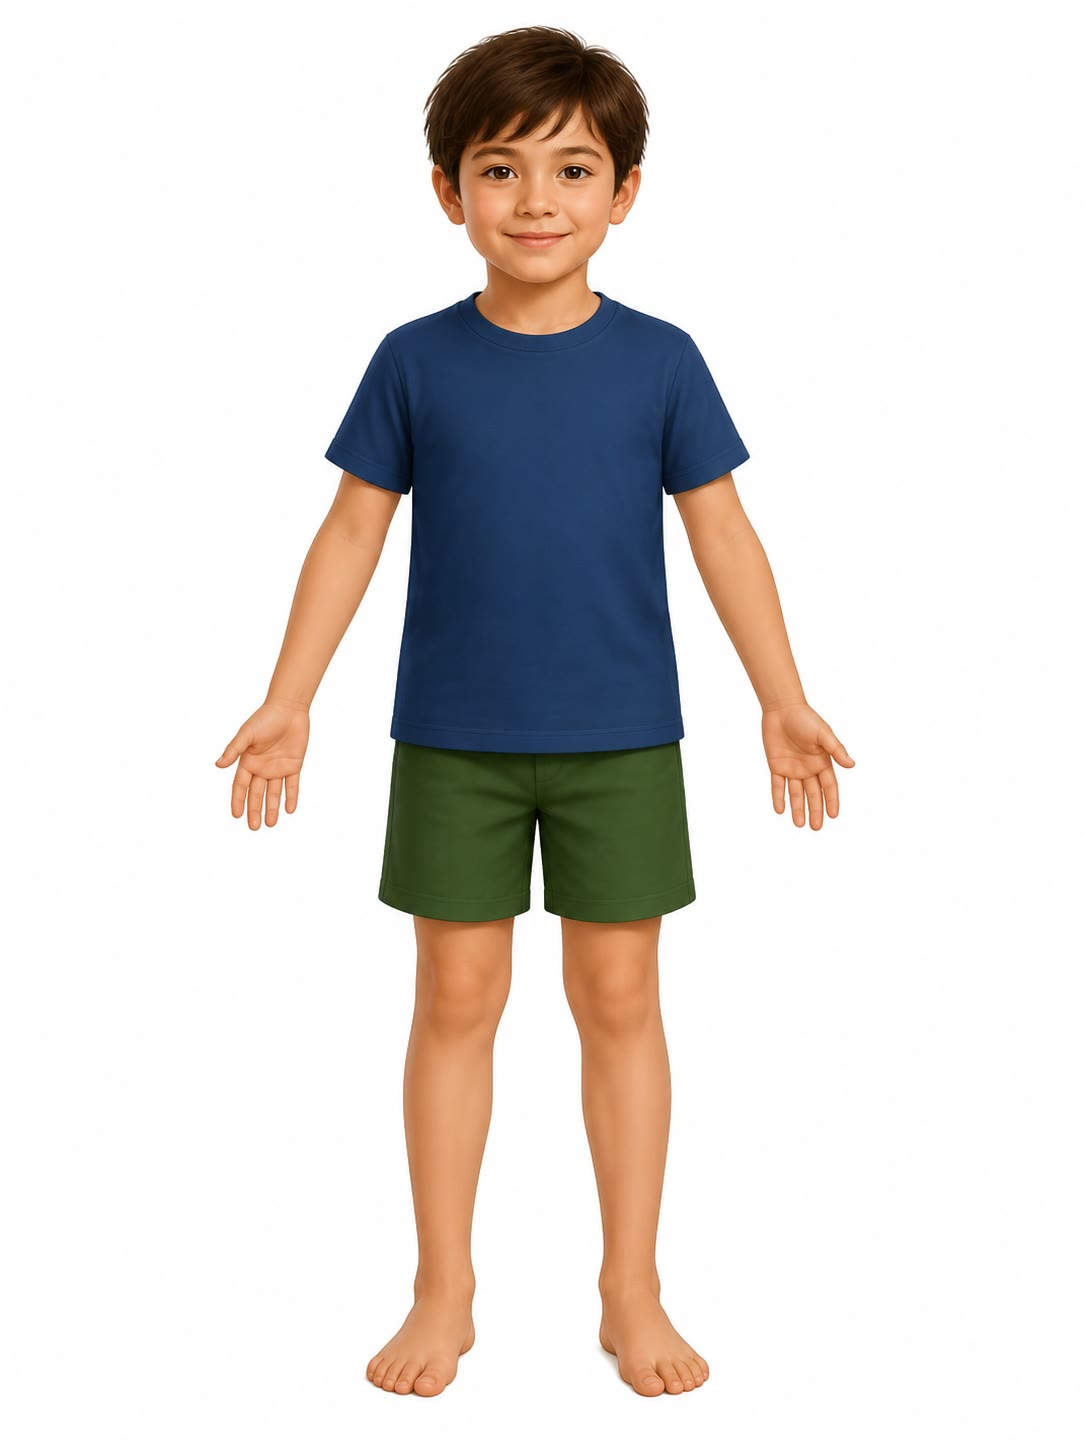
\includegraphics[width=0.42\linewidth]{images/book1/ai/fig-child-standing.jpg}};
  \begin{scope}[x={(img.south east)}, y={(img.north west)},
      every node/.style={font=\small}]
    \draw[omDef, thick] (0.57,0.90) -- (0.76,0.92) node[right] {头};
    \draw[omDef, thick] (0.53,0.80) -- (0.76,0.83) node[right] {脖子};
    \draw[omDef, thick] (0.58,0.62) -- (0.78,0.66) node[right] {树干};
    \draw[omDef, thick] (0.74,0.46) -- (0.86,0.38)
      node[below, align=center] {手臂和 \\ 手};
    \draw[omDef, thick] (0.60,0.18) -- (0.78,0.14)
      node[right, align=left] {腿和 \\ 脚};
  \end{scope}
\end{tikzpicture}

{\small 人体的三个主要部分：头、树干和
\omterm{def:g1:my-body:parts}{四肢}，\omterm{def:g1:my-body:parts}{脖子}把头与树干相连。}
\end{omfigure}

\begin{example}[和猫的结构一样吗？]\label{ex:g1:my-body:cat}
拿你和猫比一比：都有头、身体和\omterm{def:g1:my-body:parts}{四肢}，
看起来很相似。但猫用四条腿走路，你则用两条腿站立，
两只手臂空着，用来拿东西、画画和挥手。而在猫有尾巴的地方，
你却没有尾巴。
\end{example}

\section{弯曲：关节}

\begin{definition}[关节]\label{def:g1:my-body:joint}
\emph{关节}\index{关节}是身体可以弯曲
或转动的地方。\emph{肘}\index{肘}使手臂弯曲，
\emph{膝}\index{膝}使腿弯曲，
\emph{肩}\index{肩}使整条手臂转动，
\emph{腕}\index{腕}和\emph{踝}\index{踝}使
手和脚弯曲。两个关节之间，身体保持笔直。
\end{definition}

\begin{omfigure}
\begin{tikzpicture}[scale=1.0]
  % straight arm
  \draw[very thick] (0,0) -- (2.0,0);
  \draw[very thick] (2.0,0) -- (3.8,0);
  \fill[omThm] (2.0,0) circle (0.1);
  \fill[omDef!60] (0,0) circle (0.1);
  \draw[thick, fill=omDef!8] (4.0,0) circle (0.18);
  \node[below, font=\small] at (1.9,-0.3) {手臂伸直};
  % bent arm
  \begin{scope}[xshift=6.6cm]
    \draw[very thick] (0,0) -- (2.0,0);
    \draw[very thick] (2.0,0) -- (3.1,1.45);
    \fill[omThm] (2.0,0) circle (0.1);
    \fill[omDef!60] (0,0) circle (0.1);
    \draw[thick, fill=omDef!8] (3.22,1.6) circle (0.18);
    \node[below, font=\small] at (1.9,-0.3) {手臂在肘部弯曲};
    \draw[omThm] (2.05,0.12) -- (1.55,0.8)
      node[above left, font=\small, omThm] {关节在弯曲};
  \end{scope}
  \node[font=\small] at (1.0,1.4) {肩};
  \draw[omDef!60] (0.05,0.12) -- (0.55,1.15);
\end{tikzpicture}

{\small 手臂只在\omterm{def:g1:my-body:joint}{关节}处弯曲：肩（蓝色）和
肘（红色）。两者之间，手臂保持笔直。}
\end{omfigure}

\begin{example}[试一试：僵直膝盖走路]\label{ex:g1:my-body:stiff}
试着不弯曲膝盖走一走。这样也能走，
只是要迈着僵硬的小鸭步。再试着从地上
捡起一支铅笔，不弯曲膝盖、髋部或背部。\omterm{def:g1:my-body:joint}{关节}使
身体的动作流畅、敏捷又轻松。
\end{example}

\begin{remark}[左右]\label{rem:g1:my-body:sides}
身体有左右两侧，几乎像镜子一样对称：
每侧一只手臂和一条腿，头部两侧各一只眼睛、一只耳朵。
分清自己的左手和右手，也是身体的知识，
它能告诉别人你指的是哪一边。
\end{remark}

\section{我的身体在长大}

\begin{proposition}[长大]\label{prop:g1:my-body:growth}
儿童的身体会\emph{生长}\index{生长}：变得越来越高、
越来越重，一年又一年，直到长成大人的样子。生长是
缓慢而稳定的——慢得让人感觉不到，却容易测量。
\end{proposition}
\admitted

\begin{example}[门框上的刻痕]\label{ex:g1:my-body:doorframe}
站到门框旁边；大人用铅笔
在你的身高处做记号。过几个月再量一次：新的记号更高！你
从来没有感觉到自己在长高，但两道记号，一上一下，
清清楚楚地说明了这一点。
\end{example}

\begin{omfigure}
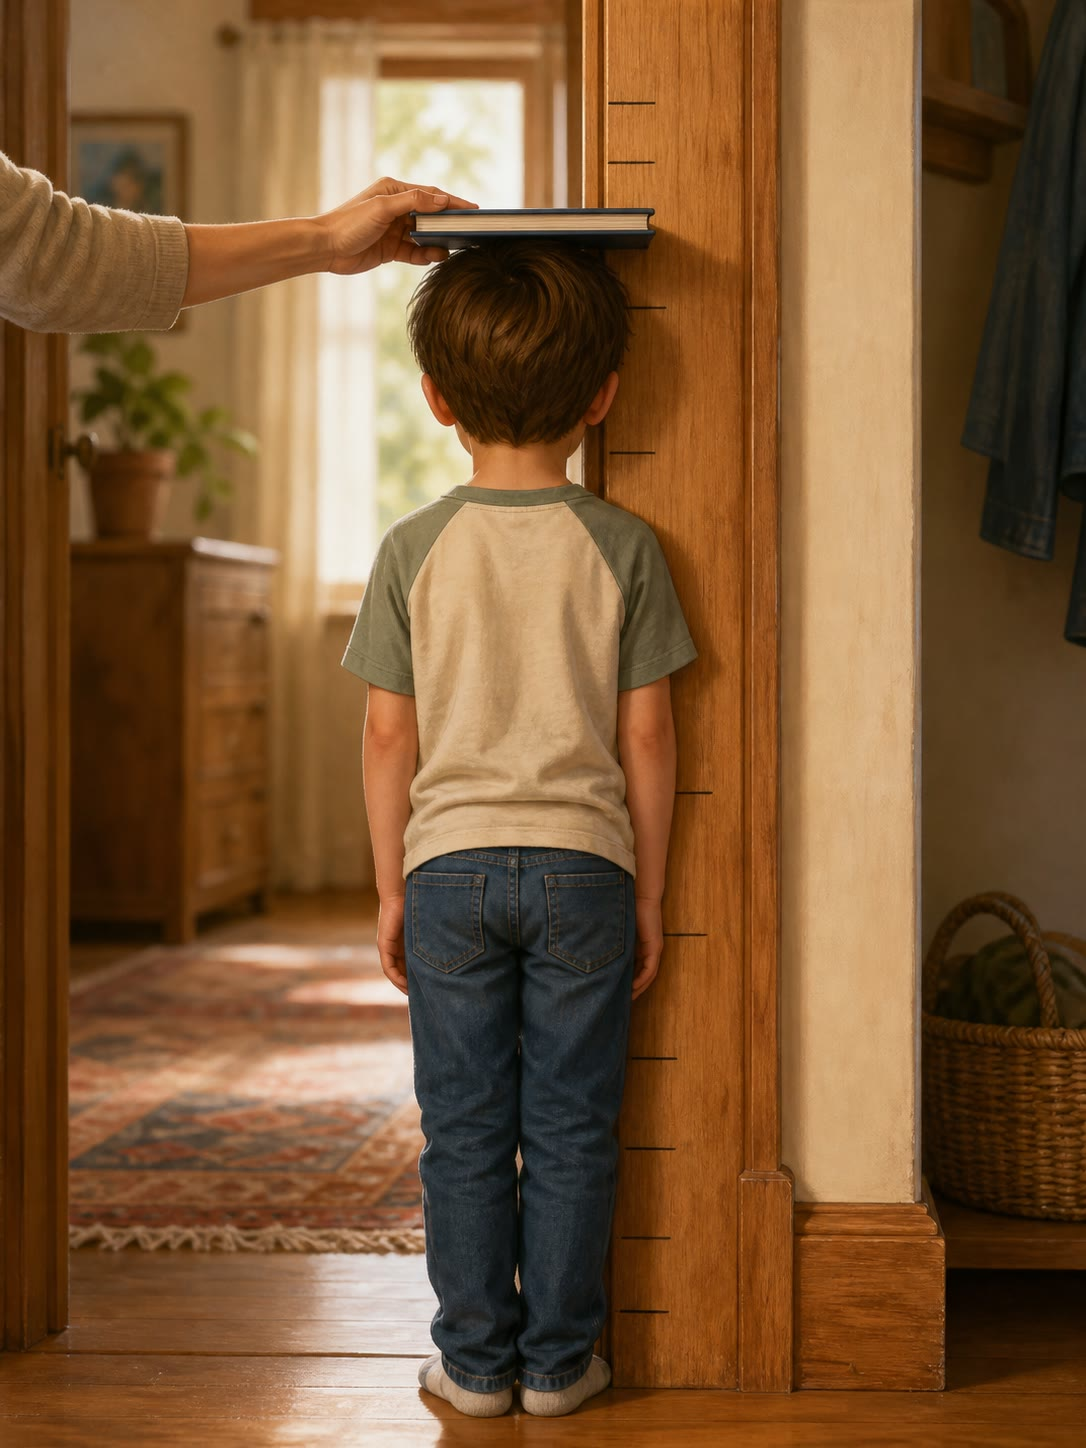
\includegraphics[width=0.46\linewidth]{images/book1/ai/g1-body-doorframe.jpg}

{\small 在门框前测量的那天：平放的书
把头顶正好压到木板上。}
\end{omfigure}

\begin{method}[测量身高]\label{met:g1:my-body:measure}
\begin{enumerate}
  \item 脱掉鞋子；
  \item 站直，背部和脚跟靠墙，目视
        前方；
  \item 帮忙的人把一本平放的书放在你的头上，保持水平，
        贴着墙面；
  \item 在书下方的位置做记号，并在旁边
        写上日期。
\end{enumerate}
每次用同样的方法测量，记号才可靠——
也才能互相比较。
\end{method}

\begin{remark}[每个人的身体都不同]\label{rem:g1:my-body:different}
同一个班里，有的孩子高一些，有的矮一些；有的孩子
长得早，有的长得晚。这些都是正常的。身体就像脸：
构造相同，却各不相同。你门框上的记号
属于你自己——它们不是用来和邻居比赛的。
\end{remark}

\section{练习}

\begin{exercise}[$\star$]\label{exo:g1:my-body:1}
说出人体的三个主要部分。什么把头和
躯干连在一起？
\end{exercise}

\begin{exercise}[$\star$]\label{exo:g1:my-body:2}
每个肢体的末端在哪里——手臂的末端是什么，以及
腿的末端是什么？
\end{exercise}

\begin{exercise}[$\star$]\label{exo:g1:my-body:3}
哪个\omterm{def:g1:my-body:joint}{关节}会弯曲：(a) 手臂中间的\omterm{def:g1:my-body:joint}{关节}？(b) 腿
中间的\omterm{def:g1:my-body:joint}{关节}？(c) 手臂末端的手？
\end{exercise}

\begin{exercise}[$\star$]\label{exo:g1:my-body:4}
用左手碰一碰右耳。你的手臂刚才用了哪些
\omterm{def:g1:my-body:joint}{关节}？至少说出两个。
\end{exercise}

\begin{exercise}[$\star$]\label{exo:g1:my-body:5}
在\cref{ex:g1:my-body:cat}中，找出一处你的身体与
猫相似之处，以及两处不同之处。
\end{exercise}

\begin{exercise}[$\star$]\label{exo:g1:my-body:6}
为什么\cref{met:g1:my-body:measure}中帮忙的人
不只是看一看，而要把平放的书放在你的头上？
\end{exercise}

\begin{exercise}[$\star$]\label{exo:g1:my-body:7}
门框上有两道记号：去年的，还有今天的，
比它稍高一点。这些记号说明了什么？你感觉到它在发生吗？
\end{exercise}

\begin{exercise}[$\star$]\label{exo:g1:my-body:8}
做\cref{ex:g1:my-body:stiff}中的僵膝走路，
然后不弯曲手肘，试着拍拍手。哪些日常动作
需要用到\omterm{def:g1:my-body:joint}{关节}？
\end{exercise}

\begin{exercise}[$\star\star$]\label{exo:g1:my-body:9}
米娅是班上最矮的，为此很担心。
根据\cref{rem:g1:my-body:different}，它怎样回答她？
\end{exercise}

\begin{exercise}[$\star\star$]\label{exo:g1:my-body:10}
用一根木棍做成的木偶不能坐在椅子上。在哪里
切断木棍并加上转折点，才能让它坐下？说出
你所切的位置所模仿的身体\omterm{def:g1:my-body:joint}{关节}。
\end{exercise}
